\section{The Main Arrangement Class\label{arr_sec:arr_class}}
%===================================

The class \ccc{Arrangement_2<Traits,Dcel>} is the main class in
the arrangement package. It is used to represent planar
arrangements and provides the interface needed to construct them,
traverse them, and maintain them. An arrangement is defined by
a geometric {\em traits} class that determines the family of planar
curves that form the arrangement, and a \dcel\ class, which
represents the {\em topological structure} of the planar subdivision.
It supplies a minimal set of geometric operations (predicates and
constructions) required to construct and maintain the arrangement
and to operate on it.

The design of the arrangement package is guided by the need to
separate between the representation of the arrangements and the
various geometric algorithms that operate on them, and by the need to
separate between the topological and geometric aspects of the planar
subdivision. The separation is exhibited by the two template
parameters of the \ccc{Arrangement_2} template:
\begin{itemize}
\item The \ccc{Traits} template-parameter should be instantiated with
a model of the \ccc{ArrangementBasicTraits_2} concept. The traits
class defines the types of $x$-monotone curves and two-dimensional
points, \ccc{X_monotone_curve_2} and \ccc{Point_2} respectively, and
supports basic geometric predicates on them.

In the first sections of this chapter we always use
\ccc{Arr_segment_traits_2} as our traits class, to construct
arrangements of line segments. However, the arrangement package 
contains several other traits classes that can handle also
polylines (continuous piecewise-linear curves), conic arcs, and arcs
of rational functions. We exemplify the usage of these traits classes
in Section~\ref{arr_sec:traits}.
\item The \ccc{Dcel} template-parameter should be instantiated with
a class that is a model of the \ccc{ArrangementDcel} concept. The
value of this parameter is \ccc{Arr_default_dcel<Traits>} by default.
However, in many applications it is necessary
to extend the \dcel\ features; see Section~\ref{arr_sec:ex_dcel} for
further explanations and examples.
\end{itemize}

\subsection{A Simple Program}
%----------------------------

\lcTex{%
  \setlength{\ArrangementTwoWidthRight}{1.6cm}
  \setlength{\ArrangementTwoWidthLeft}{\ArrangementTwoWidthLineReal}
  \addtolength{\ArrangementTwoWidthLeft}{-\ArrangementTwoWidthRight}
  \begin{minipage}{\ArrangementTwoWidthLeft}
}
\begin{ccHtmlOnly}
  <p><center>
    <img src="./fig/triangle.gif" border=0 alt="triangle" align=right>
  </center>
\end{ccHtmlOnly}
The simple program listed below constructs a planar map of three line
segments forming a triangle. The constructed arrangement is instantiated
with the \ccc{Arr_segment_traits_2} traits class to handle segments only.
The resulting arrangement consists of two faces, a bounded triangular face
and the unbounded face.
The program is not very useful as it is, since it ends immediately
after the arrangement is constructed. We give more enhanced examples
in the rest of this chapter.
\lcTex{%
  \end{minipage}\hspace{\ArrangementTwoMinipageSpace}
  \begin{minipage}{\ArrangementTwoWidthRight}
    \begin{center}
    \includegraphics{Arrangement_on_surface_2/fig/triangle}
    \end{center}
  \end{minipage}
}

\begin{alltt}
#include <CGAL/Cartesian.h>
#include <CGAL/MP_Float.h>
#include <CGAL/Quotient.h>
#include <CGAL/Arr_segment_traits_2.h>
#include <CGAL/Arrangement_2.h>

typedef CGAL::Quotient<CGAL::MP_Float>     Number_type;
typedef CGAL::Cartesian<Number_type>       Kernel;
typedef CGAL::Arr_segment_traits_2<Kernel> Traits_2;
typedef Traits_2::Point_2                  Point_2;
typedef Traits_2::X_monotone_curve_2       Segment_2;
typedef CGAL::Arrangement_2<Traits_2>      Arrangement_2;

int main()
\{
  Arrangement_2   arr;
  Segment_2       cv[3];
  Point_2         p1 (0, 0), p2 (0, 4), p3 (4, 0);
 
  cv[0] = Segment_2 (p1, p2);
  cv[1] = Segment_2 (p2, p3);
  cv[2] = Segment_2 (p3, p1);
  CGAL::insert (arr, &cv[0], &cv[3]);

  return (0);
\}
\end{alltt}

\subsection{Traversing the Arrangement\label{arr_ssec:traverse}}
%--------------------------------------

The simplest and most fundamental arrangement operations are the
various traversal methods, which allow users to systematically go
over the relevant features of the arrangement at hand.

As mentioned above, the arrangement is represented as a \dcel,
which stores three containers of vertices, halfedges and faces. Thus,
the \ccc{Arrangement_2} class supplies iterators for these
containers. For example, the methods \ccc{vertices_begin()} and
\ccc{vertices_end()} return \ccc{Arrangement_2::Vertex_iterator}
objects that define the valid range of arrangement vertices. The value
type of this iterator is \ccc{Arrangement_2::Vertex}. Moreover, the
vertex-iterator type is equivalent to
\ccc{Arrangement_2::Vertex_handle}, which serves as a pointer to a
vertex. As we show next, all functions related to arrangement features
accept handle types as input parameters and return handle types as
their output.

In addition to the iterators for arrangement vertices, halfedges
and faces, the arrangement class also provides \ccc{edges_begin()}
and \ccc{edges_end()} that return
\ccc{Arrangement_2::Edge_iterator} objects for traversing the
arrangement edges. Note that the value type of this iterator is
\ccc{Arrangement_2::Halfedge}, representing one of the twin
halfedges that represent the edge.

All iterator, circulator\footnote{A {\em circulator} is used to
traverse a circular list, such as the list of halfedges incident to
a vertex --- see below.} and handle types also have non-mutable
({\em const}) counterparts. These non-mutable iterators are useful
to traverse an arrangement without changing it. For example,
the arrangement has a
non-constant member function called \ccc{vertices_begin()} that
returns a \ccc{Vertex_iterator} object and another const member
function that returns a \ccc{Vertex_const_iterator} object. In fact,
all methods listed in this section that return an iterator, a
circulator or a handle have non-mutable counterparts. It should be
noted that, for example, \ccc{Vertex_handle} can be readily converted
into a \ccc{Vertex_const_handle}, but not vice-verse.

Conversion of a non-mutable handle to a corresponding mutable
handle are nevertheless possible, and can be performed using the
static function \ccc{Arrangement_2::non_const_handle()} (see, e.g.,
Section~\ref{arr_ssec:pl}). There are
three variant of this function, one for each type of handle.

\subsubsection{Traversal Methods for an Arrangement Vertex\label{arr_sssec:tr_vertex}}
%~~~~~~~~~~~~~~~~~~~~~~~~~~~~~~~~~~~~~~~~~~~~~~~~~~~~~~~~~~

A vertex is always associated with a geometric entity, namely with
a \ccc{Point_2} object, which can be obtained by the \ccc{point()}
method of the \ccc{Vertex} class nested within \ccc{Arrangement_2}.

The \ccc{is_isolated()} method determines whether a vertex is isolated
or not. Recall that the halfedges incident to a non-isolated vertex,
namely the halfedges that share a common target vertex, form a circular
list around this vertex. The \ccc{incident_halfedges()} method returns
a circulator of type \ccc{Arrangement_2::Halfedge_around_vertex_circulator}
that enables the traversal of this circular list in a clockwise
direction. The value type of this circulator is \ccc{Halfedge}.

The following function prints all the neighbors of a given
arrangement vertex (assuming that the \ccc{Point_2} type can be
inserted into the standard output using the \ccc{<<} operator). The
arrangement type is the same as in the simple example above.
\begin{alltt}
void print_neighboring_vertices (Arrangement_2::Vertex_const_handle v)
\{
  if (v->is_isolated()) \{
    std::cout << "The vertex (" << v->point() << ") is isolated" << std::endl;
    return;
  \}

  Arrangement_2::Halfedge_around_vertex_const_circulator first, curr;
  first = curr = v->incident_halfedges();

  std::cout << "The neighbors of the vertex (" << v->point() << ") are:";
  do \{
    // Note that the current halfedge is directed from u to v:
    Arrangement_2::Vertex_const_handle u = curr->source();
    std::cout << " (" << u->point() << ")";
  \} while (++curr != first);
  std::cout << std::endl;
\}
\end{alltt}

In case of an isolated vertex, it is possible to obtain the face
that contains this vertex using the \ccc{face()} method.

\subsubsection{Traversal Methods for an Arrangement Halfedge\label{arr_sssec:tr_halfedge}}
%~~~~~~~~~~~~~~~~~~~~~~~~~~~~~~~~~~~~~~~~~~~~~~~~~~~~~~~~~~~~

Each arrangement edge, realized as a pair of twin halfedges,
is associated with an \ccc{X_monotone_curve_2} object, which
can be obtained by the \ccc{curve()} method of the \ccc{Halfedge}
class nested in the \ccc{Arrangement_2} class.

The \ccc{source()} and \ccc{target()} methods return handles to
the halfedge source and target vertices respectively. We can
obtain a handle to the twin halfedge using the \ccc{twin()}
method. From the definition of halfedges, it follows that if
\ccc{he} is a halfedge handle, then:
\begin{itemize}
\item \ccc{he->curve()} is equivalent to \ccc{he->twin()->curve()},
\item \ccc{he->source()} is equivalent to \ccc{he->twin()->target()}, and
\item \ccc{he->target()} is equivalent to \ccc{he->twin()->source()}.
\end{itemize}

Every halfedge has an incident face that lies to its left, which
can be obtained by the \ccc{face()} method. Recall that a
halfedge is always one link in a connected chain of halfedges that
share the same incident face, known as a {\em CCB}. The
\ccc{prev()} and \ccc{next()} methods return handles to the
previous and next halfedges in the CCB respectively. 
%(note that \ccc{he->prev()} is not necessarily equivalent to
%\ccc{he->twin()->next()}).

As the CCB is a circular list of halfedges, it is only natural to 
traverse it using a circulator. The \ccc{ccb()} method returns a 
\ccc{Arrangement_2::Ccb_halfedge_circulator} object for the
halfedges along the CCB.

The function \ccc{print_ccb()} listed below prints all $x$-monotone
curves along a given CCB (assuming that the \ccc{Point_2} and the
\ccc{X_monotone_curve_2} types can be inserted into the standard output
using the \ccc{<<} operator).
\begin{alltt}
void print_ccb (Arrangement_2::Ccb_halfedge_const_circulator circ)
\{
  Ccb_halfedge_const_circulator curr = circ;
  std::cout << "(" << curr->source()->point() << ")";
  do \{
    Arrangement_2::Halfedge_const_handle he = curr->handle();
    std::cout << "   [" << he->curve() << "]   "
              << "(" << he->target()->point() << ")";
  \} while (++curr != circ);
  std::cout << std::endl;
\}
\end{alltt}

\subsubsection{Traversal Methods for an Arrangement Face\label{arr_sssec:tr_face}}
%~~~~~~~~~~~~~~~~~~~~~~~~~~~~~~~~~~~~~~~~~~~~~~~~~~~~~~~~

An arrangement of bounded curves always has a single unbounded face.
The function \ccc{unbounded_face()} returns a handle to this face.
(Note that an empty arrangement contains nothing {\em but} the
unbounded face.)

Given a \ccc{Face} object, we can use the \ccc{is_unbounded()}
method to determine whether it is unbounded. Bounded faces have an
outer CCB, and the \ccc{outer_ccb()} method returns a circulator
for the halfedges along this CCB. Note that the halfedges along
this CCB wind in a counterclockwise orientation around the outer
boundary of the face.

A face can also contain disconnected components in its interior,
namely holes and isolated vertices:
\begin{itemize}
\item The \ccc{holes_begin()} and \ccc{holes_end()} methods return
\ccc{Arrangement_2::Hole_iterator} iterators that define the range
of holes inside the face. The value type of this iterator is
\ccc{Ccb_halfedge_circulator}, defining the CCB that winds in a
clockwise orientation around a hole.
\item The \ccc{isolated_vertices_begin()} and
\ccc{isolated_vertices_end()} methods return
\ccc{Arrangement_2::Isolated_vertex_iterator} iterators that
define the range of isolated vertices inside the face. The value
type of this iterator is \ccc{Vertex}.
\end{itemize}

The function \ccc{print_face()} listed below prints the outer and
inner boundaries of a given face, using the function \ccc{print_ccb()},
which was introduced in the previous subsection.
\begin{alltt}
void print_face (Arrangement_2::Face_const_handle f)
\{
  // Print the outer boundary.
  if (f->is_unbounded())
    std::cout << "Unbounded face. " << std::endl;
  else \{
    std::cout << "Outer boundary: ";
    print_ccb (f->outer_ccb());
  \}

  // Print the boundary of each of the holes.
  Arrangement_2::Hole_const_iterator hi;
  int                                 index = 1;
  for (hi = f->holes_begin(); hi != f->holes_end(); ++hi, ++index) \{
    std::cout << "    Hole #" << index << ": ";
    print_ccb (*hi);
  \}

  // Print the isolated vertices.
  Arrangement_2::Isolated_vertex_const_iterator iv;
  for (iv = f->isolated_vertices_begin(), index = 1;
       iv != f->isolated_vertices_end(); ++iv, ++index)
  \{
    std::cout << "    Isolated vertex #" << index << ": "
              << "(" << iv->point() << ")" << std::endl;
  \}
\}
\end{alltt}

\subsubsection{Additional Example\label{arr_sssec:tr_ex}}
%~~~~~~~~~~~~~~~~~~~~~~~~~~~~~~~~~

The function listed below prints the current setting of a given
arrangement. This concludes the preview of the various traversal
methods.\footnote{The file \ccc{arr_print.h}, which can be
found under the examples folder, includes this function and the
rest of the functions listed in this section. Over there they are
written in a more generic fashion, where the arrangement type
serves as a template parameter for these functions, so different
instantiations of the \ccc{Arrangement_2<Traits,Dcel>} template
can be provided to the same function templates.}
\begin{alltt}
void print_arrangement (const Arrangement_2& arr)
\{
  // Print the arrangement vertices.
  Vertex_const_iterator vit;
  std::cout << arr.number_of_vertices() << " vertices:" << std::endl;
  for (vit = arr.vertices_begin(); vit != arr.vertices_end(); ++vit) \{
    std::cout << "(" << vit->point() << ")";
    if (vit->is_isolated())
      std::cout << " - Isolated." << std::endl;
    else
      std::cout << " - degree " << vit->degree() << std::endl;
  \}

  // Print the arrangement edges.
  Edge_const_iterator eit;
  std::cout << arr.number_of_edges() << " edges:" << std::endl;
  for (eit = arr.edges_begin(); eit != arr.edges_end(); ++eit)
    std::cout << "[" << eit->curve() << "]" << std::endl;

  // Print the arrangement faces.
  Face_const_iterator fit;
  std::cout << arr.number_of_faces() << " faces:" << std::endl;
  for (fit = arr.faces_begin(); fit != arr.faces_end(); ++fit)
    print_face (fit);
\}
\end{alltt}

\subsection{Modifying the Arrangement\label{arr_ssec:modify}}
%-------------------------------------

In this section we review the various member functions of the
\ccc{Arrangement_2} class that allow users to modify the
topological structure of the arrangement by introducing new edges
or vertices, modifying them, or removing them.

The arrangement member-functions that insert new curves into the
arrangement, thus enabling the construction of a planar subdivision, are
rather specialized, as they require a-priori knowledge on the location of
the inserted curve. Indeed, for most purposes it is more convenient to
construct an arrangement using the free (global) insertion-functions.

\subsubsection{Inserting Non-Intersecting $x$-Monotone Curves\label{arr_sssec:mf_insert_cv}}
%~~~~~~~~~~~~~~~~~~~~~~~~~~~~~~~~~~~~~~~~~~~~~~~~~~~~~~~~~~~~~

The most important functions that allow users to modify the
arrangement, and perhaps the most frequently used ones, are the
specialized insertion functions of $x$-monotone curves whose
interior is disjoint from any other curve in the existing
arrangement and do not contain any vertex of the arrangement. In
addition, these function require that the location of the curve in the
arrangement is known.

The motivation behind these rather harsh restrictions on the nature of
the inserted curves is the decoupling of the topological arrangement
representation from the various algorithms that operate on it. While
the insertion of an $x$-monotone curve whose interior is disjoint from
all existing arrangement features is quite straightforward (as we show
next), inserting curves that intersect with the curves already inserted
into the arrangement is much more complicated and requires the
application of non-trivial geometric algorithms.
These insertion operations are therefore implemented as free functions
that operate on the arrangement and the inserted curve(s); see
Section~\ref{arr_sec:gl_funcs} for more details and
examples.\footnote{You may skip to Section~\ref{arr_sec:gl_funcs},
and return to this subsection at a later point in time.}

\begin{figure}[t]
\begin{ccTexOnly}
  \begin{center}
  \begin{tabular}{ccc}
    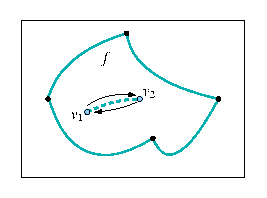
\includegraphics{Arrangement_on_surface_2/fig/insert_in_face} &
    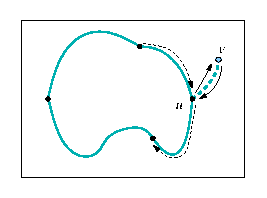
\includegraphics{Arrangement_on_surface_2/fig/insert_from_vertex} &
    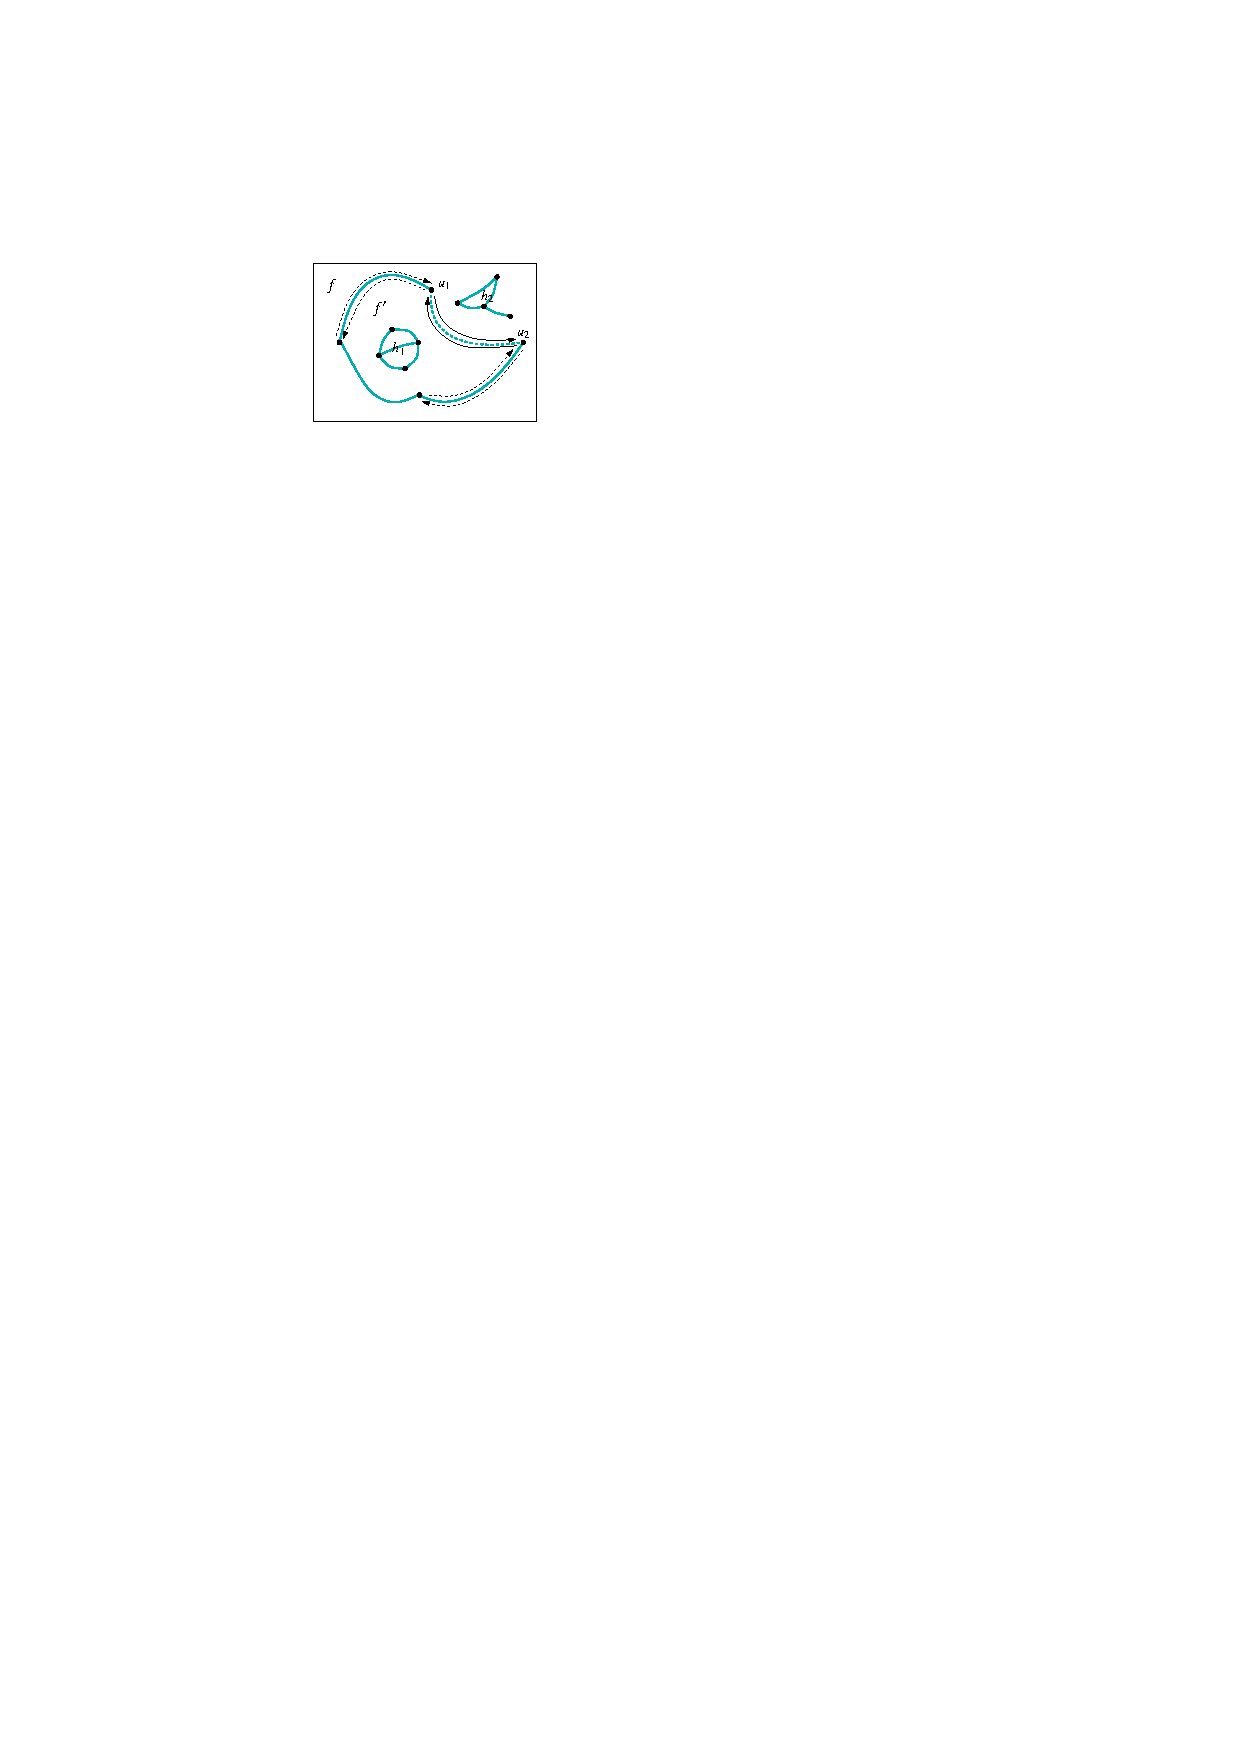
\includegraphics{Arrangement_on_surface_2/fig/insert_at_vertices}\\
  {\small (a)} & {\small (b)} & {\small (c)}\\
  \end{tabular}
  \end{center}
\end{ccTexOnly}
\begin{ccHtmlOnly}
  <p><center>
    <img src="./fig/insert.gif" border=0 alt="insert">
  </center>
\end{ccHtmlOnly}
\caption{The various specialized insertion procedures. The
inserted $x$-monotone curve is drawn with a light dashed line,
surrounded by two solid arrows that represent the pair of twin
half-edges added to the \dcel. Existing vertices are shown as
black dots while new vertices are shown as light dots. Existing
half-edges that are affected by the insertion operations are drawn
as dashed arrows. (a) Inserting a curve as a new hole inside the
face $f$. (b) Inserting a curve from an existing vertex $u$ that
corresponds to one of its endpoints. (c) Inserting an $x$-monotone
curve whose endpoints are the already existing vertices
$u_1$ and $u_2$. In our case, the new pair of half-edges close a
new face $f'$, where the hole $h_1$, which used to belong to $f$,
now becomes an enclave in this new face.} \label{arr_fig:insert}
\end{figure}

When an $x$-monotone curve is inserted into an existing arrangement, such
that the interior of this curve is disjoint from any arrangement feature,
only the following three scenarios are possible, depending on the status
of the endpoints of the inserted subcurve:
\begin{enumerate}
%
\item In case both curve endpoints do not correspond to any existing
arrangement vertex we have to create two new vertices
corresponding to the curve endpoints and connect them using a pair
of twin halfedges. This halfedge pair initiates a new hole inside
the face that contains the curve in its interior.
%
\item If exactly one endpoint corresponds to an existing arrangement
vertex (we distinguish between a vertex that corresponds to the left
endpoint of the inserted curve and a vertex corresponding to its right
endpoint), we have to create a new vertex that corresponds to the other
endpoint of the curve and to connect the two vertices by a pair of
twin halfedges that form an ``antenna'' emanating from the boundary
of an existing connected component (note that if the existing vertex
used to be isolated, this operation is actually equivalent to forming
a new hole inside the face that contains this vertex).

\lcTex{%
  \setlength{\ArrangementTwoWidthRight}{4.1cm}
  \setlength{\ArrangementTwoWidthLeft}{\ArrangementTwoWidthLineReal}
  \addtolength{\ArrangementTwoWidthLeft}{-\ArrangementTwoWidthRight}
  \begin{minipage}{\ArrangementTwoWidthLeft}
}
\item
\begin{ccHtmlOnly}
  <p><center>
    <img src="./fig/connect_comp.gif" border=0 alt="connect_comp" align=right>
  </center>
\end{ccHtmlOnly}
If both endpoints correspond to existing arrangement
vertices, we connect these vertices using a pair of twin halfedges.
(If one or both vertices are isolated this case reduces to one of
the two previous cases respectively.) The two following subcases may
occur:
\begin{itemize}
\item Two disconnected components are merged into a single connected
component (as is the case with the segment $s_1$ in the figure to the
left).
%
\item A new face is created, a face that splits from an existing
arrangement face. In this case we also have to examine the holes and
isolated vertices in the existing face and move the relevant ones
inside the new face (as is the case with the segment $s_2$ in the
figure to the left).
\end{itemize}
\lcTex{%
  \end{minipage}%\hspace{\ArrangementTwoMinipageSpace}
  \begin{minipage}{\ArrangementTwoWidthRight}
    \begin{center}\hspace{\ArrangementTwoMinipageSpace}
    \includegraphics{Arrangement_on_surface_2/fig/connect_comp}
    \end{center}
  \end{minipage}
}
\end{enumerate}

The \ccc{Arrangement_2} class offers insertion functions named
\ccc{insert_in_face_interior()}, \ccc{insert_from_left_vertex()},
\ccc{insert_from_right_vertex()} and \ccc{insert_at_vertices()}
that perform the special insertion procedures listed above. The
first function accepts an $x$-monotone curve $c$ and an arrangement
face $f$ that contains this curve in its interior. The other
functions accept an $x$-monotone curve $c$ and handles to the existing
vertices that correspond to the curve endpoint(s). Each of the four
functions returns a handle to one of the twin halfedges that have
been created, where:
\begin{itemize}
\item \ccc{insert_in_face_interior(c, f)} returns a halfedge directed
from the vertex corresponding to the left endpoint of \ccc{c}
toward the vertex corresponding to its right endpoint.
%
\item \ccc{insert_from_left_vertex(c, v)} and
\ccc{insert_from_right_vertex(c, v)} returns a halfedge whose
source is the vertex $v$ that and whose target is the new vertex
that has just been created.
%
\item \ccc{insert_at_vertices(c, v1, v2)} returns a halfedge directed
from $v_1$ to $v_2$.
\end{itemize}

\begin{figure}[t]
\begin{ccTexOnly}
  \begin{center}
  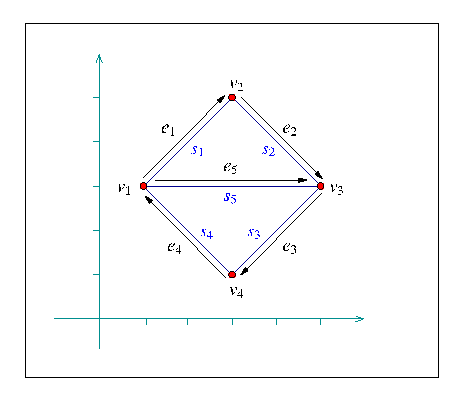
\includegraphics{Arrangement_on_surface_2/fig/ex_1}
  \end{center}
\end{ccTexOnly}
\begin{ccHtmlOnly}
  <p><center>
  <img src="./fig/ex_1.gif" border=0 alt="Example 1">
  </center>
\end{ccHtmlOnly}
\caption{The arrangement of the line segments $s_1, \ldots, s_5$
constructed in \ccc{edge_insertion.cpp}. The arrows mark the direction of
the halfedges returned from the various insertion
functions.\label{arr_fig:ex_1}}
\end{figure}

The following program demonstrates the usage of the four insertion
functions. It creates an arrangement of five line segments, as
depicted in Figure~\ref{arr_fig:ex_1}.\footnote{Notice that in all
figures in the rest of this chapter the coordinate axes are drawn
only for illustrative purposes and are {\em not} part of the
arrangement.} As the arrangement is very
simple, we use the simple Cartesian kernel of \cgal\ with integer
coordinates for the segment endpoints. We also use the 
\ccc{Arr_segment_traits_2} class that enables the efficient
maintenance of arrangements of line segments; see more details on
this traits class in Section~\ref{arr_sec:traits}. This example, as
many others in this chapter, uses some print-utility functions from
the file \ccc{print_arr.h}; these functions are also listed in
Section~\ref{arr_ssec:traverse}.

\ccIncludeExampleCode{Arrangement_on_surface_2/edge_insertion.cpp}

Observe that the first line segment is inserted in the interior of
the unbounded face. The other line segments are inserted
using the vertices created by the insertion of previous segments.
The resulting arrangement consists of three faces, where the two
bounded faces form together a hole in the unbounded face.

\subsubsection{Manipulating Isolated Vertices\label{arr_sssec:mf_iso_verts}}
%~~~~~~~~~~~~~~~~~~~~~~~~~~~~~~~~~~~~~~~~~~~~~~~~

Isolated points are in general simpler geometric entities than
curves and indeed the member functions that manipulate them are
easier to understand.

The function \ccc{insert_in_face_interior(p, f)} inserts an
isolated point $p$, located in the interior of a given face $f$,
into the arrangement and returns a handle to the arrangement
vertex it has created and associated with $p$. Naturally, this
function has a precondition that $p$ is really an isolated point,
namely it does not coincide with any existing arrangement vertex
and does not lie on any edge. As mentioned in
Section~\ref{arr_ssec:traverse}, it is possible to obtain the face
containing an isolated vertex handle $v$ by calling \ccc{v->face()}.

The function \ccc{remove_isolated_vertex(v)} receives a handle to
an isolated vertex and removes it from the arrangement.

\begin{figure}[t]
\begin{ccTexOnly}
  \begin{center}
  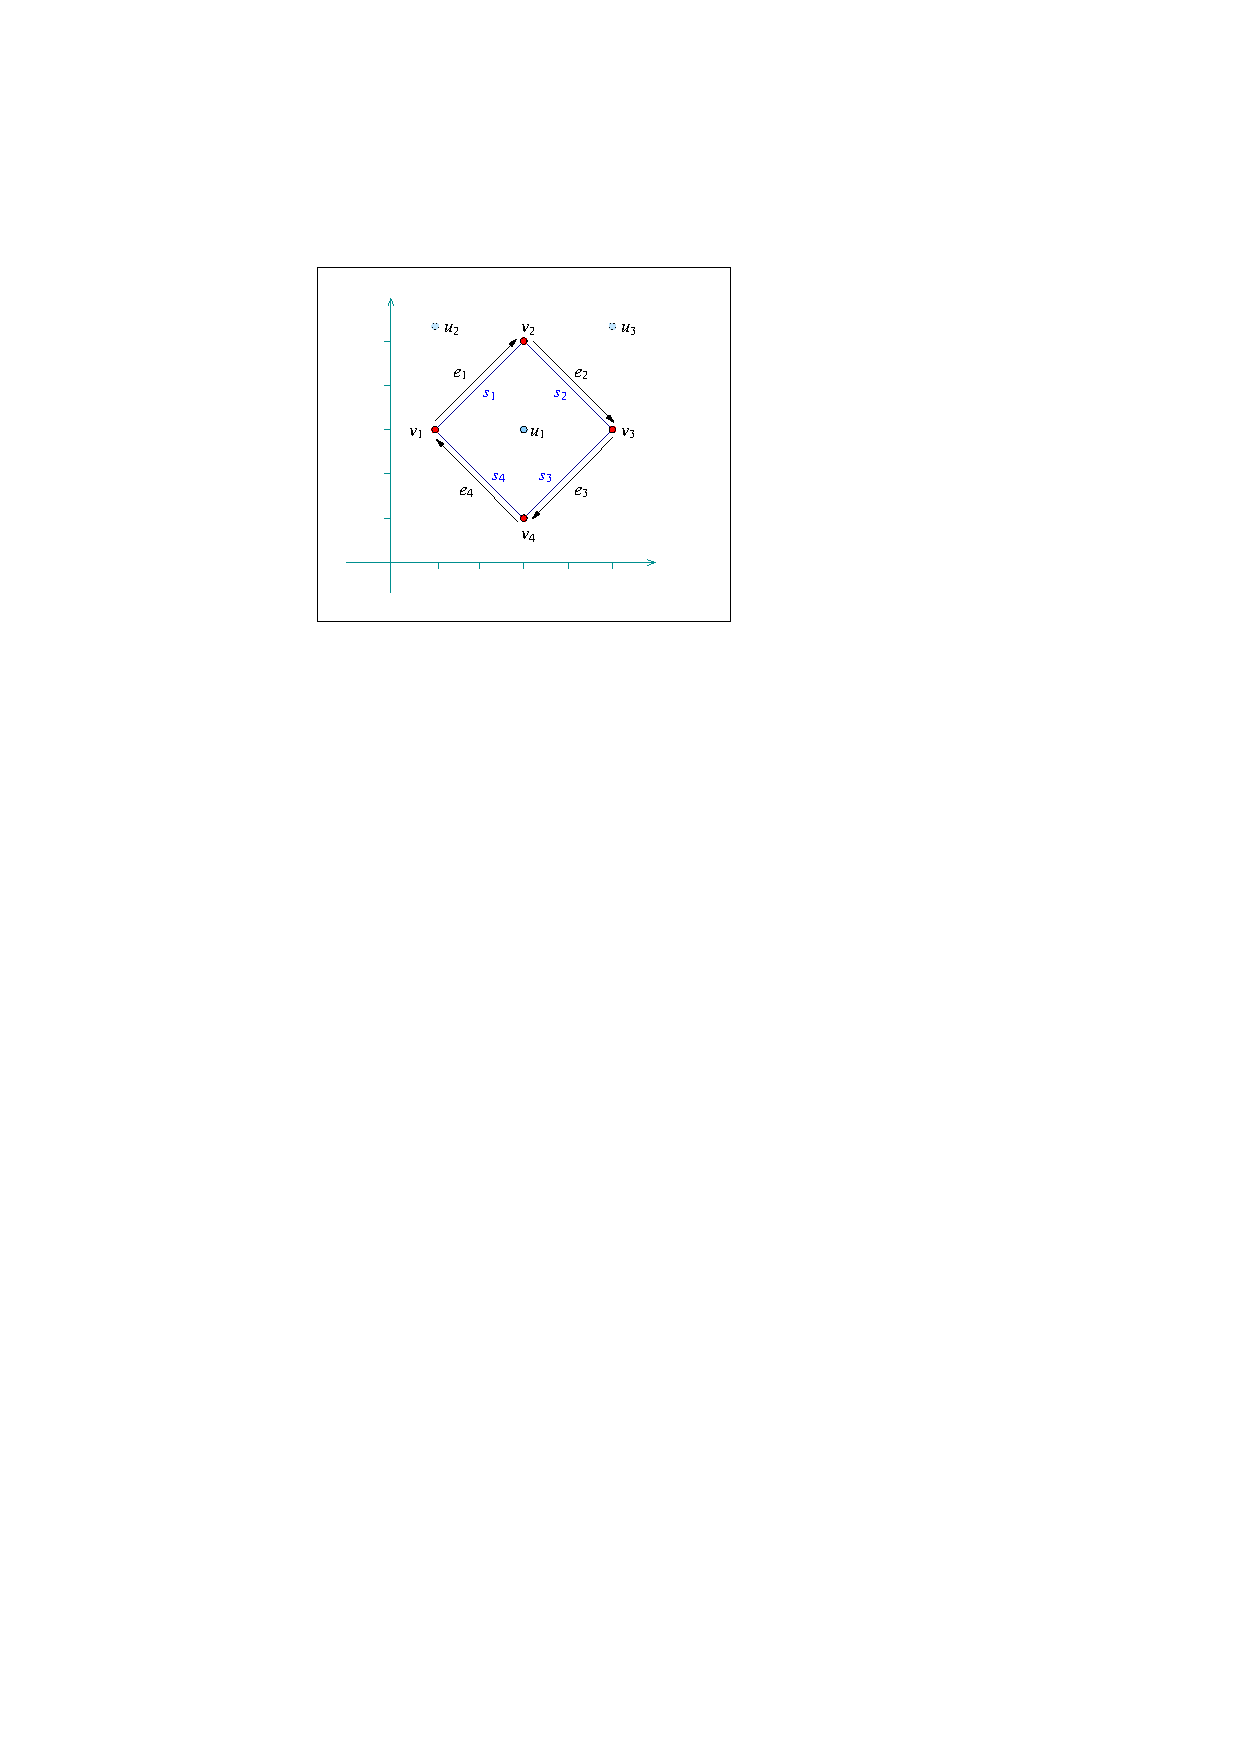
\includegraphics{Arrangement_on_surface_2/fig/ex_2}
  \end{center}
\end{ccTexOnly}
\begin{ccHtmlOnly}
  <p><center>
  <img src="./fig/ex_2.gif" border=0 alt="Example 2">
  </center>
\end{ccHtmlOnly}
\caption{An arrangement of line segments containing three isolated
vertices, as constructed in \ccc{isolated_vertices.cpp}. The vertices $u_2$
and $u_3$ are eventually removed from the arrangement.\label{arr_fig:ex_2}}
\end{figure}

The following program demonstrates the usage of the arrangement
member-functions for manipulating isolated vertices. It first
inserts three isolated vertices located inside the unbounded face, then
it inserts four line segments that form a rectangular hole inside the
unbounded face (see Figure~\ref{arr_fig:ex_2} for an
illustration). Finally, it traverses the vertices and removes those
isolated vertices that are still contained in the unbounded face
($u_2$ and $u_3$ in this case):

\ccIncludeExampleCode{Arrangement_on_surface_2/isolated_vertices.cpp}

\subsubsection{Manipulating Halfedges\label{arr_sssec:mf_halfedges}}
%~~~~~~~~~~~~~~~~~~~~~~~~~~~~~~~~~~~~~~~~~~~~~~~~

In the previous subsection we showed how to introduce new isolated
vertices in the arrangement. But how does one create a vertex that
lies on an existing arrangement edge (more precisely, on an
$x$-monotone curve that is associated with an arrangement edge)?

It should be noted that such an operation involves the splitting
of a curve at a given point in its interior, while the traits
class used by \ccc{Arrangement_2} does not necessarily have the
ability to perform such a split operation. However, if users have
the ability to split an $x$-monotone curve into two at a given point
$p$ (this is usually the case when employing a more sophisticated
traits class; see Section~\ref{arr_sec:traits} for more details)
they can use the \ccc{split_edge(e, c1, c2)} function, were
$c_1$ and $c_2$ are the two subcurves resulting from splitting the
$x$-monotone curve associated with the halfedge $e$ at some point
(call it $p$) in its interior. The function splits the halfedge pair into two
pairs, both incident to a new vertex $v$ associated with $p$, and
returns a handle to a halfedge whose source equals $e$'s source
vertex and whose target is the new vertex $v$.

The reverse operation is also possible. Suppose that we have a
vertex $v$ of degree $2$, whose two incident halfedges, $e_1$ and
$e_2$, are associated with the curves $c_1$ and $c_2$. Suppose
further that it is possible to merge these two curves into a single
continuous $x$-monotone curve $c$. Calling \ccc{merge_edge(e1, e2, c)}
will merge the two edges into a single edge associated with the curve
$c$, essentially removing the vertex $v$ from the arrangement.

Finally, the function \ccc{remove_edge(e)} removes the edge $e$
from the arrangement. Note that this operation is the reverse of
an insertion operation, so it may cause a connected
component to split into two, or two faces to merge into one, or a
hole to disappear. By default, if the removal of \ccc{e} causes one
of its end-vertices to become isolated, we remove this vertex as well.
However, users can control this behavior and choose to keep the
isolated vertices by supplying additional Boolean flags to
\ccc{remove_edge()} indicating whether the source and the target vertices
are to be removed should they become isolated.

\begin{figure}[t]
\begin{ccTexOnly}
  \begin{center}
  \begin{tabular}{ccc}
    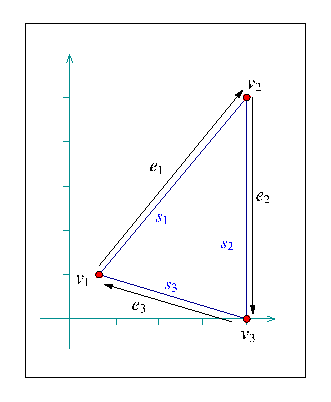
\includegraphics{Arrangement_on_surface_2/fig/ex_3a} &
    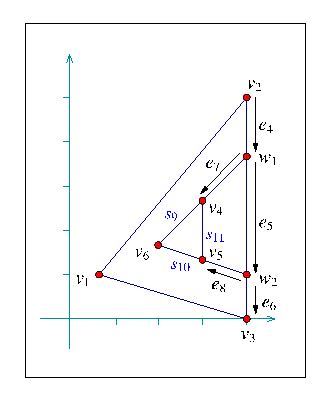
\includegraphics{Arrangement_on_surface_2/fig/ex_3b} &
    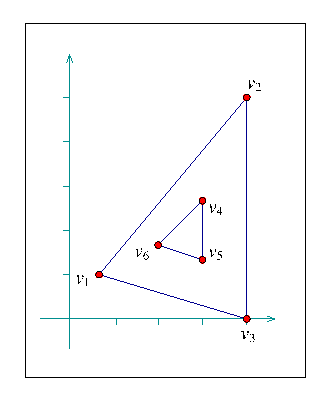
\includegraphics{Arrangement_on_surface_2/fig/ex_3c} \\
  {\small (a)} & {\small (b)} & {\small (c)}\\
  \end{tabular}
  \end{center}
\end{ccTexOnly}
\begin{ccHtmlOnly}
  <p><center>
  <img src="./fig/ex_3.gif" border=0 alt="Example 3">
  </center>
\end{ccHtmlOnly}
\caption{An arrangement of line segments as constructed
in \ccc{edge_manipulation.cpp}. Note that the edges $e_7$ and $e_8$ and the
vertices $w_1$ and $w_2$, introduced in step~(b) are eventually
removed in step~(c).\label{arr_fig:ex_3}}
\end{figure}

In the following example program we show how the edge-manipulation
functions can be used. The program works in three
steps, as demonstrated in Figure~\ref{arr_fig:ex_3}. Note that
here we still stick to integer coordinates, but as we work on a
larger scale we use an unbounded integer number-type (in this
case, the \ccc{Gmpz} type taken from the {\sc Gmp} library)
instead of the built-in \ccc{int} type.\footnote{As a rule of
thumb, one can use a bounded integer type for representing line
segments whose coordinates are bounded by
$\lfloor\sqrt[3]{M}\rfloor$, where $M$ is the maximal
representable integer value. This guarantees that no overflows
occur in the computations carried out by the traits class, hence
all traits-class predicates always return correct results.} 
In case the {\sc Gmp} library is not installed (as indicated by
the \ccc{CGAL_USE_GMP} flag defined in \ccc{CGAL/basic.h}), we
use \ccc{MP_Float}, a number-type included in \cgal's support
library that is capable of storing floating-point numbers with
unbounded mantissa. We also use the standard Cartesian
kernel of \cgal\ as our kernel. This is recommended when the
kernel is instantiated with a more complex number type, as we
demonstrate in other examples in this chapter.

\ccIncludeExampleCode{Arrangement_on_surface_2/edge_manipulation.cpp}

Note how we use the halfedge handles returned from
\ccc{split_edge()} and \ccc{merge_edge()}. Also note the insertion
of the isolated vertex $v_6$ located inside the triangular face (the
incident face of $e_7$). This vertex seizes from being isolated, as it
is gets connected to other vertices.

In this context, we should mention the two member functions
\ccc{modify_vertex(v, p)}, which sets $p$ to be the point
associated with the vertex $v$, and \ccc{modify_edge(e, c)}, which
sets $c$ to be the $x$-monotone curve associated with the halfedge
$e$. These functions have preconditions that $p$ is
geometrically equivalent to \ccc{v->point()} and $c$ is equivalent
to \ccc{e->curve()} (i.e., the two curves have the same graph),
respectively, to avoid the invalidation of the geometric structure of
the arrangement. At a first glance it may seen as these two functions
are of little use. However, we should keep in mind that there may be
extraneous data (probably non-geometric) associated with the point
objects or with the curve objects, as defined by the traits class. With
these two functions we can modify this data; see more details in
Section~\ref{arr_sec:traits}.

In addition, we can use these functions to replace a geometric
object (a point or a curve) with an equivalent object that has a
more compact representation. For example, we can replace the point
$(\frac{20}{40}, \frac{99}{33})$ associated with some vertex $v$,
by $(\frac{1}{2}, 3)$.

\newpage
\begin{ccAdvanced}
\subsubsection{Advanced Insertion Functions\label{arr_sssec:adv_insert}}
%~~~~~~~~~~~~~~~~~~~~~~~~~~~~~~~~~~~~~~~~~~~

\lcTex{%
  \setlength{\ArrangementTwoWidthRight}{2.5cm}
  \setlength{\ArrangementTwoWidthLeft}{\ArrangementTwoWidthLineReal}
  \addtolength{\ArrangementTwoWidthLeft}{-\ArrangementTwoWidthRight}
  \begin{minipage}{\ArrangementTwoWidthLeft}
}
\begin{ccHtmlOnly}
  <p><center>
    <img src="./fig/pred_around_vertex.gif" border=0 alt="pred_around_vertex" align=right>
  </center>
\end{ccHtmlOnly}
Assume that the specialized insertion function
\ccc{insert_from_left_vertex(c,v)} is invoked for a curve $c$,
whose left endpoint is already associated with a non-isolated
vertex $v$.  Namely, $v$ has already several incident halfedges. It
is necessary in this case to locate the exact place for the
new halfedge mapped to the inserted new curve $c$ in the circular
list of halfedges incident to $v$. More precisely, it is sufficient
to locate one of the halfedges \ccc{pred} directed toward $v$ such
that $c$ is located between \ccc{pred} and \ccc{pred->next()} in
clockwise order around $v$, in order to complete the insertion
(see Figure~\ref{arr_fig:insert} for an illustration). This may
take $O(d)$ time where $d$ is the degree of the vertex. However,
if the halfedge \ccc{pred} is known in advance, the insertion can
be carried out in constant time.
\lcTex{%
  \end{minipage}\hspace{\ArrangementTwoMinipageSpace}
  \begin{minipage}{\ArrangementTwoWidthRight}
    \begin{center}
    \includegraphics{Arrangement_on_surface_2/fig/pred_around_vertex}
    \end{center}
  \end{minipage}
}

The \ccc{Arrangement_2} class provides the advanced versions of
the specialized insertion functions for a curve $c$ --- namely we have
\ccc{insert_from_left_vertex(c,pred)} and
\ccc{insert_from_right_vertex(c,pred)} that accept a halfedge \ccc{pred}
as specified above, instead of a vertex $v$. These functions are
more efficient, as they take constant time and do not perform any
geometric operations. Thus, they should be used when the halfedge
\ccc{pred} is known. In case that the vertex $v$ is isolated or
that the predecessor halfedge for the new inserted curve is not
known, the simpler versions of these insertion functions should be
used.

Similarly, there exist two overrides of the
\ccc{insert_at_vertices()} function: One that accept the two
predecessor halfedges around the two vertices $v_1$ and $v_2$ that
correspond to the curve endpoints, and one that accepts a handle
for one vertex and a predecessor halfedge around the other
vertex.

\begin{figure}[t]
\begin{ccTexOnly}
  \begin{center}
  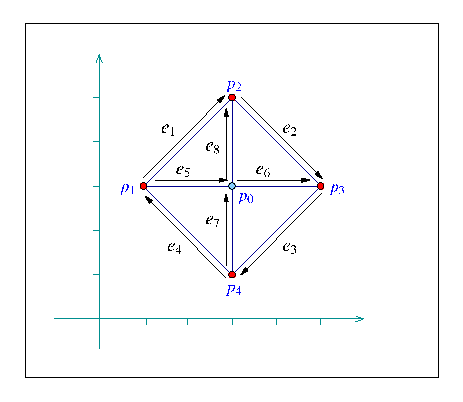
\includegraphics{Arrangement_on_surface_2/fig/ex_4}
  \end{center}
\end{ccTexOnly}
\begin{ccHtmlOnly}
  <p><center>
  <img src="./fig/ex_4.gif" border=0 alt="Example 4">
  </center>
\end{ccHtmlOnly}
\caption{An arrangement of line segments, as constructed in
\ccc{special_edge_insertion.cpp}. Note that $p_0$ is initially inserted
as an isolated point and later on connected to the other four
vertices.\label{arr_fig:ex_4}}
\end{figure}

The following program shows how to construct the arrangement
depicted in Figure~\ref{arr_fig:ex_4} using the specialized
insertion functions that accept predecessor halfedges:

\ccIncludeExampleCode{Arrangement_on_surface_2/special_edge_insertion.cpp}

It is possible to perform even more refined operations on an
\ccc{Arrangement_2} instance given specific topological information.
As most of these operations are very fragile and perform no precondition
testing on their input in order to gain efficiency, they are not included
in the public interface of the arrangement class. Instead, the
\ccc{Arr_accessor<Arrangement>} class allows access to these internal
arrangement operations --- see more details in the Reference Manual.
\end{ccAdvanced}
